\documentclass[twoside]{esi-tfg}
\usepackage{custom}
\usepackage{epigraph}

%% -- Información general --
\title{Alcaudon: Streaming data platform}
\author{Francisco Fernández Castaño}{}


%% -- Variables de la clase esi-tfg --

%- datos del autor

%\address{}
%\city{}
%\country{}
\email{francisco.fernandez.castano@gmail.com}
\phone{645999999}
% \homepage{http://esi.uclm.es/~juan.nadie}


%- datos del documento

%\logo{informatica.pdf}
\advisorFirst{Dr. David Villa Alises}
\advisorDepartment{Departamento de Tecnologías y Sistemas de la Información}

\docdate{2017}{September}
\intensification{Computation}
%\license{Texto de licencia al gusto de cada uno.}


\begin{document}

\cover
\bastardtitle
\frontpage

\frontmatter
\copyrightpage
\jury

\chapter{Resumen}


\chapter{Abstract}

Currently, the amount of collected data is growing. Internet companies track all
user actions in order to provide better experiences. Science experiments
generate colossal amounts of data. Another growing source of data is Internet
of Things, i.e. autonomous cars need to collect and analyze large amounts of
data in order to function properly. These, combined with the plunging cost of
data storage makes storing large amounts of information for later analysis very
compelling.

Organizations should take advantage of all these data in order to overcome
ad-hoc business decisions in favor of data-driven approaches. Therefore, to
satisfy data analysis needs, many data processing systems have appeared in
the last years. Those systems were focused on processing large amounts of
historical data. However, there is an increasing need to acquire knowledge
from data as soon as possible, allowing a prompt reaction to a wide range of
events.

This project aims to implement a distributed streaming data processing platform,
Alcaudon, allowing near real-time data analysis of unbounded data-sets. One of
the objectives of this project is to provide a powerful programming model,
making it straightforward to write distributed data analysis pipelines.
Moreover, Alcaudon has been designed contemplating scalability and
fault-tolerance. Therefore, this projects presents a robust and potent tool to
process and analyze unbounded data-sets.


\chapter{Greetings}

Thanks for reading this.
\quoteauthor{Francisco}

\dedication{To my parents and Yolanda}
\epigraph{Computational processes are abstract beings that inhabit computers. As they evolve, processes manipulate other abstract things called data. The evolution of a process is directed by a pattern of rules called a program. People create programs to direct processes. In effect, we conjure the spirits of the computer with our spells.}{--- \textup{Hal Abelson}, Structure and Interpretation of Computer Programs}


\tableofcontents
\listoftables
\listoffigures
\lstlistoflistings
\chapter{List of acronyms}

{\small
\begin{acronym}[XXXXXXXX]
  \acro{UUID}     {Universally unique identifier}
  \acro{ADT}     {Algebraic Data Type}
\end{acronym}
}


\mainmatter

\chapter{Introduction}
\label{chap:introduction}

\drop{T}{oday} each of Facebook, Twitter and Linkedin~\cite{facebook, twitter, linkedin}
ingest more than 12M events per second. Another important automated data source
is Internet of Things~\cite{iot} that is bringing even larger volumes of data
that are predicted to double every year. The plunging cost of data storage,
accelerated by cloud computing, is enabling many companies to collect and store
huge amounts of data. The analysis and exploration of these data sets can change
ad-hoc business decisions to data-driven ones, with higher probability of being
successful.

\noindent
There are many scenarios where data analysis can play a big role:

Web companies do \textit{behavioral analytics} so they can study how their customers use
their platforms. This enables actions like \textit{session targeting}. This consists of
special offers depending on what the customer is doing while using the service,
increasing the chances of successful commercial transactions.

Another related action could be \textit{campaign optimization}. One of the biggest
business in internet is advertising. Companies that are able to generate the best
return for the advertisers are the ones that will overcome the competition.

New technological architectures, like microservices-based, provide solutions to
problems that before were almost impossible to solve, such as scalability. There is
a cost associated with this architecture: monitoring these services. Companies
like Netflix have thousands of services running~\cite{netflix}, and some of those
services can produce over 40.000 metrics per second. Analyzing metrics data is
key to being able to detect anomalies, degradation in services and without doubt
the only way to run large distributed systems.

But it does not end here, as there are many more examples where data analytics
is fundamental. Scientific experiments, i.e. CERN (generates terabytes of data, per
experiment)~\cite{cern}, security, and many more that are arising over time.

\begin{figure}[!h]
\begin{center}
\includegraphics[width=1\textwidth]{mapreduce.jpg}
\caption{Map-Reduce architecture~\cite{mapreduce}}
\label{fig:mapreduce}
\end{center}
\end{figure}

Traditional DBMS cannot cope with the scale and heterogeneity of the data sets
cited previously. Over time, models like MapReduce~\cite{mapreduce}
Figure~\ref{fig:mapreduce}, Spark~\cite{spark} and Storm appeared. Those
architectural models facilitated the parallelization of data analysis processes
at scale, running on commodity hardware. These systems are classified as batch
processing, meaning that all input should be collected into a batch before
processing it.

MapReduce and batch processing paradigms have been quite successful over the
years on large data-sets scenarios. But new needs are arising
and data analysts are becoming more demanding with their requirements. Batch
systems are designed to run with bounded data, imposing big latencies. In some
situations it is not feasible to wait hours to get back results from analytics.
One example could be monitoring microservices architectures where anomalies must
be investigated and fixed as soon as possible to avoid service disruptions.

To avoid latencies imposed by batch systems, hybrid systems were designed. One
paradigmatic example is Lambda Architecture~\cite{lambda}. It consists of
two data processing systems running in parallel. One of the systems, known as
streaming system, will provide approximate results in nearly real time. To
obtain more precise results, a classic batch systems run over the same data-set.
Soon, these systems showed many problems. Running two processing pipelines in
parallel is translated into many operational issues as well as more costs~\cite{kappa}.

In general, batch processing systems don't perform well on stream data-sets.
Stream data-sets, as defined in~\cite{streamissues}, can be characterized as follows:
%
\textit{
\begin{itemize}
\item The data elements in the stream arrive online.
\item The system has no control over the order in which data elements arrive to
  be processed, either within a data stream or across data streams.
\item Data streams are potentially unbounded in size.
\item Once an element from a data stream has been processed it is discarded or
  archived — it cannot be retrieved easily unless it is explicitly stored in
  memory, which typically is small relative to the size of the data streams
\end{itemize}
}

It is clear that batch systems were one of the enablers of big processing pipelines,
but new data processing platforms are needed. In particular, data processing platforms
that are able to deal with stream data.

To overcome the limitations imposed by batch systems on streaming data, a few
alternatives appeared. Google developed MillWheel~\cite{millwheel} and Google
DataFlow~\cite{dataflow}. Those systems were designed with the previously presented
problems in mind. The main differentiator was how unordered data was treated. To
facilitate working with unordered events, the next concepts were introduced~\cite{dataflow}:
\textit{
  \begin{itemize}
  \item Windowing: slicing data into finite chunks for processing.
  \item Triggering: stimulating the output of a specific window at a grouping operation.
  \end{itemize}
}

This project will be focused on developing a data processing system using the
same principles that Google Dataflow and MillWheel are based on.

During the next chapters a description of the specific objectives of this
project, an exposition of the state of the art and the methodology used to
develop this project will be presented. Once these topics are introduced, a
detailed characterization of Alcaudon architecture is explained as well as the
accomplished results.

% Local Variables:
% ispell-local-dictionary: "american"
% End:

\chapter{Objectives}
\label{chap:objectives}

\drop{I}{n} this chapter, the global objectives that have motivated the project
are described. As well as the more specific goals that want to be achieved.

\section{General Objectives}

The purpose of this project is to develop a distributed, fault-tolerant and
elastic streaming processing framework aimed for unbounded datasets. Given a
user defined topology of computations, the system will place them into a cluster
of nodes optimizing the resource utilization. Alcaudon abstracts away all the
difficulties involved in programming in a distributed environment. The user just
needs to define the computations, using the Alcaudon computation Interface, data
dependencies, and the system will take care of the execution. The system should be
easily deployed into cloud platforms such as Amazon Web Services, so it can cope
with bursts of load dynamically.

\section{Specific objectives}

Given the previous general description, objectives can be categorized into the
following sub-objectives.

\subsection{Provide an abstraction to create distributed computations}
One of the primary goals of this project is to provide abstractions to create
distributed streaming programs without distributed systems expertise. To achieve
this, Alcaudon should provide a computation API that allows clients to write
their business logic without knowing any details of the underlying
infrastructure.
Alcaudon should provide means to work with persistent state in user code. A
State API is provided to work with key-value pairs.

\subsection{Develop mechanisms to ensure exactly-once processing of records}

One of the biggest problems in distributed systems is to guarantee that a record
has been delivered and processed. The system will ensure that messages are
delivered exactly-once, without any change in user code.

To achieve exactly-once delivery in a performant manner, i.e., without two-phase
commits (citation needed), Alcaudon will enforce idempotency using probabilistic
data structures and state journaling.

\subsection{Provide tools to work with out-of-order data}

Unordered data is a reality in distributed environments. Some systems enforce
monotonicity of event time using the injection time instead of the event
generation time. Alcaudon will provide tools to work with non monotonic event
times.

\subsection{Implement a cluster scheduler}

Users of Alcaudon provide a directed acyclic graph of computations. Those
tasks should be placed into the cluster available resources. Cluster scheduling
usually leads to an NP-hard problem. The system will implement a scheduler based
on heuristics to set the tasks into the computing nodes.


\subsection{Allow extensibility of sources and sinks}
Some implementations for unbounded data sources, like TCP sockets, scala collections
and twitter will be available. But users will be able to extend Alcaudon to add
custom Sources and Sinks.

\subsection{Design and implement an elastic, fault-tolerant and scalable distributed architecture}
The system should have the properties described in the reactive manifesto(citation needed):

\begin{itemize}
  \item The system should be \textit{resilient}, meaning that in the face of a failure it should keep running.
  \item The system should be \textit{elastic}, in the face of an increase of load it
    should be responsive allowing adding new resources to cope with the new
    requirements.
\end{itemize}

It should make easy to add new nodes to the cluster, so the resources available
can change depending on the needs. This design towards a more cloud oriented
architecture could facilitate offering Alcaudon as a service.

\subsection{Provide tools for observability}

The project should be designed with observability in mind. Metrics and logging
should be exposed. This allows an easier operability, giving the site
reliability engineers tools to reason about the behaviour of the system.

\chapter{State of the art}
\label{chap:stateoftheart}

\drop{T}{his} chapter aims to explain the concepts and techniques in which
Alcaudon is based on. As shown in Figure~\ref{fig:mindmap}. the project has foundations in
distributed systems, job scheduling, library design and data processing. In the
next sections, those concepts will be analyzed in more depth.

\begin{figure}[!h]
\begin{center}
\includegraphics[width=1\textwidth]{mindmap.pdf}
\caption{Alcaudon foundations}
\label{fig:mindmap}
\end{center}
\end{figure}

\section{Data Processing}

According to a recent study by \FIXME{cita y referencia juntas no
  quedan bien} Cisco~\cite{ciscosurvey}~\ref{fig:ciscodata}
data storage is growing by 40\% yearly. This implies that that by 2020
datacenters will store over 1000 ExaBytes of information. Keeping that data in
silos without performing any use of it is a poor investment.

\begin{figure}[!h]
\begin{center}
\includegraphics[width=0.8\textwidth]{ciscodata.png}
\caption{Actual Data Stored in Data Centers~\cite{ciscosurvey}}
\label{fig:ciscodata}
\end{center}
\end{figure}

Processing those amounts of data using traditionals RDBMS is not practical, as
they are not designed to work with that large load of data. In the last years
there have been many ongoing efforts on providing tools to process and analyze
large volumes of data. Some examples could be MapReduce~\cite{mapreduce},
Spark~\cite{spark} and many others. Before those frameworks appeared, there were
some systems capable of processing large amounts of data, like the
supercomputers or HPC. One of the main drawbacks of HPC is accessibility to
those high end computers. Acquiring a new \FIXME{por qué en
  mayúscula?} Supercomputer in the event of a peak
on data production is not feasible. For companies, making an investment in a
super computer is a big risk that in some cases will not be reverted as profit.
Another interesting point to make is that Supercomputers perform well many
floating-point operations per second. However, in general, the computations
executed in systems like MapReduce are simple strings manipulation, counting and
so on. Given these usage patterns, it seems that supercomputers are more suited
to perform scientific analysis.

Once the limitations of HPC for \textit{big data} scenarios have been described,
it is possible to explore how modern internet companies are using computing
resources to process data. For new organizations, it is more sensible to take
advantage of commodity hardware to process large amounts of data. One of the
reasons is that there are many tools to distribute data processing among large
clusters of commodity machines. Once that job is done, those machines can be
turned off or used for other purposes. Working with those systems provides
flexibility, both in resource usage and innovation capacity.

Even though systems such as Map-Reduce have been quite useful to
process large amounts of data, they start to have limitations in
certain aspects. Currently, the need of low latency in data processing
is getting mandatory. Organizations need to get insights about their
data as soon as possible, in order to react quickly to new trends. The
systems described previously are classified as batch systems, as they
are oriented to process historical datasets and not \textit{real time
  data}. There have been some adaptations to these systems, using
approaches like micro-batching where data is processed in smaller
batches, however the latency is still big. These new needs for data
processing have lead to the design and development of systems
specialized in unbounded data processing. These systems try to reduce
the time between the event generation and its processing. \FIXME
{deberías evitar referencias a Alcaudon en este capítulo. Estás
  contando lo que hay para usarlo como argumento para la necesidad del
  nuevo proyecto. Un estado del arte debe tener valor en si mismo
  aunque no escribieras nada más} Alcaudon fits in this category of
data processing systems, as one of its aims is being able to process
unbounded data sets with low latency.

\subsection{Cloud Computing}

Cloud computing might be seen as a recent development. However, during the 1990s
researchers at Xerox PARC started to develop ideas around what they named
\textit{ubiquitous computing}. The idea was to have computing devices
interconnected and exchanging data about almost everything. This idea was ahead
of his time because there were just a few networks around. And devices such as
cameras and microphones were still quite big, etc. Even though if this definition is
translated to 2017 seems to fit quite perfectly on how devices behave nowadays.
Cars, fridges, watches, smartphones and anything that can have a network
interface is connected to the internet. Huge amounts of data are being published
and stored into the what is now known as \textit{the cloud}. There is not a
clear definition for what \textit{cloud computing} is. For the purposes of this
text, cloud computing could be defined as a pool of shared computing and storage
resources that can be provisioned and released on demand. Given the huge amounts
of data that users store into the \textit{cloud}, companies need to outsource
computing and storing capacity, since building datacenters is a huge investment.
In the last decade, computing infrastructure offering has changed radically.

Companies such as Amazon Web Services are able to offer servers, storage and
services on demand at scale, from 1 server to 1 million servers. Having the
ability to start and stop servers on demand has democratized the ability to
process large amounts of data for many organizations. For example, a startup can
kickoff with just one server to process data. Once the business starts growing,
it can take advantage of the elasticity provided by cloud computing services,
and start using more servers to cope with the load. This is one of the reasons why
data processing systems should be designed to scale out as there are more
computing needs.
Alcaudon, as an elastic data processing system, will be able to adapt to
different loads as the computing needs increase. It will be able to use more
computing resources dynamically as more servers are added to the pool.

\section{Distributed systems}
\label{subsection:distsys}

Distributed systems can be defined as a set of computer programs,
executing on one or more computers, and coordinating actions by
exchanging \textit{messages}~\cite{GuideReliable}. Those computers are
usually located in a \textit{computer network}, a collection of
computers interconnected by hardware that supports message passing and
implement routing protocols. But if this definition is taken to the
extreme, a modern multi-core processor can be characterized as a
distributed system, with many components exchanging information in a
network and coordinating actions to get work done. To some extent, it
is possible to see distributed systems as a super set of concurrent
systems.

A more common example of a distributed system is a user requesting a web page to
a server with his smartphone. This example is a typical \textit{client-server}
model. This \textit{simple} action involves the interaction of various services
such as DNS servers, load balancers, HTTP proxies and servers. All these
services use a network as a mean to interchange messages as shown in figure
~\ref{fig:client-server}.

\begin{figure}[!h]
\begin{center}
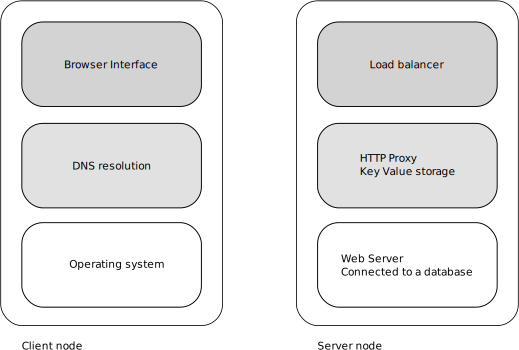
\includegraphics[width=0.7\textwidth]{client-server.pdf}
\caption{Client-server architecture}
\label{fig:client-server}
\end{center}
\end{figure}

As it has been previously discussed, distributed systems are very
common nowadays. They are present in fields like database systems,
internet of things, data processing and many more. There are some
reasons that make more convenient to work with distributed systems,
but the main reason is ability to scale. As defined
in~\cite{cloudadmin}:
%
\begin{quote}
  A system's ability to scale is its ability to process a growing workload,
  usually measured in transactions per second, amount of data or number of
  users.
\end{quote}

\begin{figure}[!h]
\begin{center}
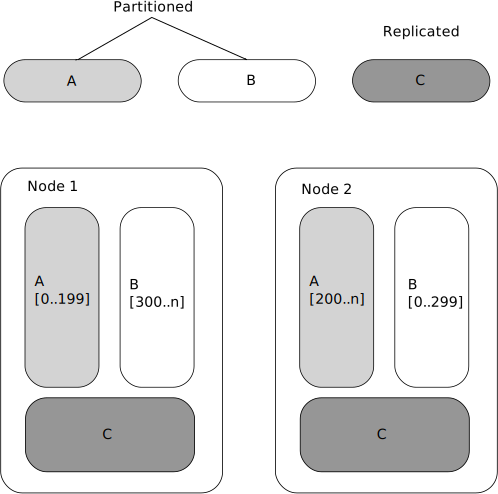
\includegraphics[width=0.7\textwidth]{partition-rep.pdf}
\caption{Partitioning and Replication}
\label{fig:partitioning}
\end{center}
\end{figure}

Distributed programming can help designing systems with the ability to scale given
the following properties:
%
\begin{itemize}
\item \textit{Reliability}: Achieved by \textit{replication} and/or
  \textit{partitioning} as illustrated in Figure ~\ref{fig:partitioning}.
\item \textit{Elasticity}: Since the systems are designed to work in
  coordination with other processes, it is possible to add more resources to
  handle increasing workloads. But there is an upper limit imposed by the
  coordination model used.
\item \textit{Parallelism}: This is a natural outcome of having multiple resources, they
  can get work done in parallel.
\item \textit{Price/performance ratio}: Scaling vertically (using more powerful
  compute nodes), has upper limits both in available technology and in costs. As
  shown in Figure ~\ref{fig:highend} the performance gap between a high end
  server and a cluster of commodity hardware nodes is tolerable. Another factor
  to take into account when distributed systems are used is the cost of
  networking communications, as it implies an overhead.
\end{itemize}

\begin{figure}[!h]
\begin{center}
\includegraphics[width=1\textwidth]{scalingcost.png}
\caption{Performance advantage of a cluster built with large SMP server nodes
  (128-core SMP) over a cluster with the same number of processor cores built
  with low-end server nodes (four-core SMP), for clusters of varying
  size~\cite{Datacenter}}[\FIXME{pon un caption breve aquí para el LOF}]
\label{fig:highend}
\end{center}
\end{figure}

\subsection{Taxonomy of a distributed system}

Once described what distributed systems are and why they are useful, it is
possible to define a taxonomy of distributed systems topics such as coordination
algorithms, global state collection, distributed consensus, etc.

As it can be seen the topic is wide, so for this documents only
\textit{distributed snapshots}, \textit{membership protocols} and \textit{time
  in distributed systems} will be covered.

\begin{itemize}
\item \textit{Time in distributed systems}:
  Programmers are used to think in sequential programs, where computation steps
  are executed one after the other. The reality in distributed and concurrent
  systems is quite different. Knowledge about global state among all the nodes
  in the system is likely to be outdated. A naive solution to this problem is
  using synchronization based on wall clocks. However, the notion of
  synchronized clocks among nodes is impractical. Protocols like \ac{NTP}~\cite{ntp}
  can have skews up to 1000 seconds, an unacceptable time in some cases. Google
  makes heavy use of hardware-assisted time synchronization using GPS clocks and
  atomic clocks to ensure global consistency for their database
  Spanner~\cite{180268} that can drift up to 100ms. Given the exposed facts, the
  only assumption that can be taken about distributed operations is that they are partially
  ordered. A formal definition for partial order is ~\cite{book:lattices}:
  \begin{definition}{(Partial order)}
    Let $P$ be a set. An order (or partial order) on $P$ is a binary relation
    $\leq$ on $P$ such that, for all $x$, $y$, $z \in P$,
    \begin{enumerate}
    \item $x \leq x$
    \item $x \leq y$ and $y \leq x$ imply $y$
    \item $x \leq y$ and $y \leq z$ imply $x \leq z$
    \end{enumerate}
  \end{definition}
  Given the exposed facts, message order in distributed systems is partial.
  However, there are algorithms that focuses on maintaining a global total order
  of operations~\cite{vclocks}. In environments where the message flow is unbounded
  the notion of completeness is weak. There is no guarantee about when all the
  messages up to a moment $T_n$ have been received or processed. To deal with
  this, Alcaudon uses watermark heuristics. A watermark heuristic defines that up
  to the instant $T_i$ there are high chances that all messages up to that point
  have been received.
\item \textit{Distributed snapshots}:
  Since Alcaudon aims to be a fault-tolerant system, guarantees about persistent
  state must be enforced. To design a resilient system, persistent state
  snapshots should be taken. There are distributed algorithms to deal with this
  problem such as Chandy-Lamport algorithm~\cite{lampsnapshot}. In general, those algorithms are focused
  on taking a global state snapshot that given the constraints presented in the
  previous section is a hard problem to solve. In Alcaudon this obstacle is
  solved by taking snapshots by computation. There is no need of a global
  snapshot since persistent state is local to each computation.

\item \textit{Membership protocols}: Another crucial aspect on an elastic
  distributed system is how to handle cluster membership. It is possible to
  classify them into two categories: static membership and dynamic membership.
  Static membership has a fixed list of cluster members that do not change along
  the life of the cluster. With this static membership there is a chance that at
  some point in time, some members of the cluster will not be available. Since
  cluster membership image is static, thew will be seen as accessible. The other
  approach is to use dynamic membership. It consists on having initial knowledge
  about a subset of the available nodes and later on, via gossiping
  protocols~\cite{gossip} new nodes can \textit{join} the cluster. This mechanism
  is also able to handle when nodes become \textit{unavailable}. For Alcaudon
  the latter membership category is more suitable. Since one of the goals is to
  provide elasticity, in this case the system will be able to be scaled in the
  need of more computing power.
\end{itemize}

\subsection{CRDT}

One of the problems when building distributed systems is sharing state among
different participants. In order to provide a global vision of shared state,
replication~\cite{book:replication} algorithms have been developed during the last
years. Nevertheless, these algorithms have certain limitations in terms of
performance and scalability due to serialization. Eric Brewer postulated the
conjecture that it is impossible for a distributed system to provide
consistency, availability and partition-tolerance guarantees. Where
they can be defined as:

\begin{itemize}
\item \textit{Consistency}: A global total order of operations is provided,
  meaning that all nodes see the same data.
\item \textit{Availability}: The system is able to respond to requests even in
  the presence of partial failures.
\item \textit{Partition tolerance}: The system is able to continue operating in
  the event of network failures.
\end{itemize}

This conjecture was proved~\cite{capproof} later and it is known nowadays as the CAP
theorem(\ref{fig:cap}). This theorem establishes a trade-off between consistency (total order
of operations) and partition-tolerance.

\begin{figure}[!h]
  \centering
  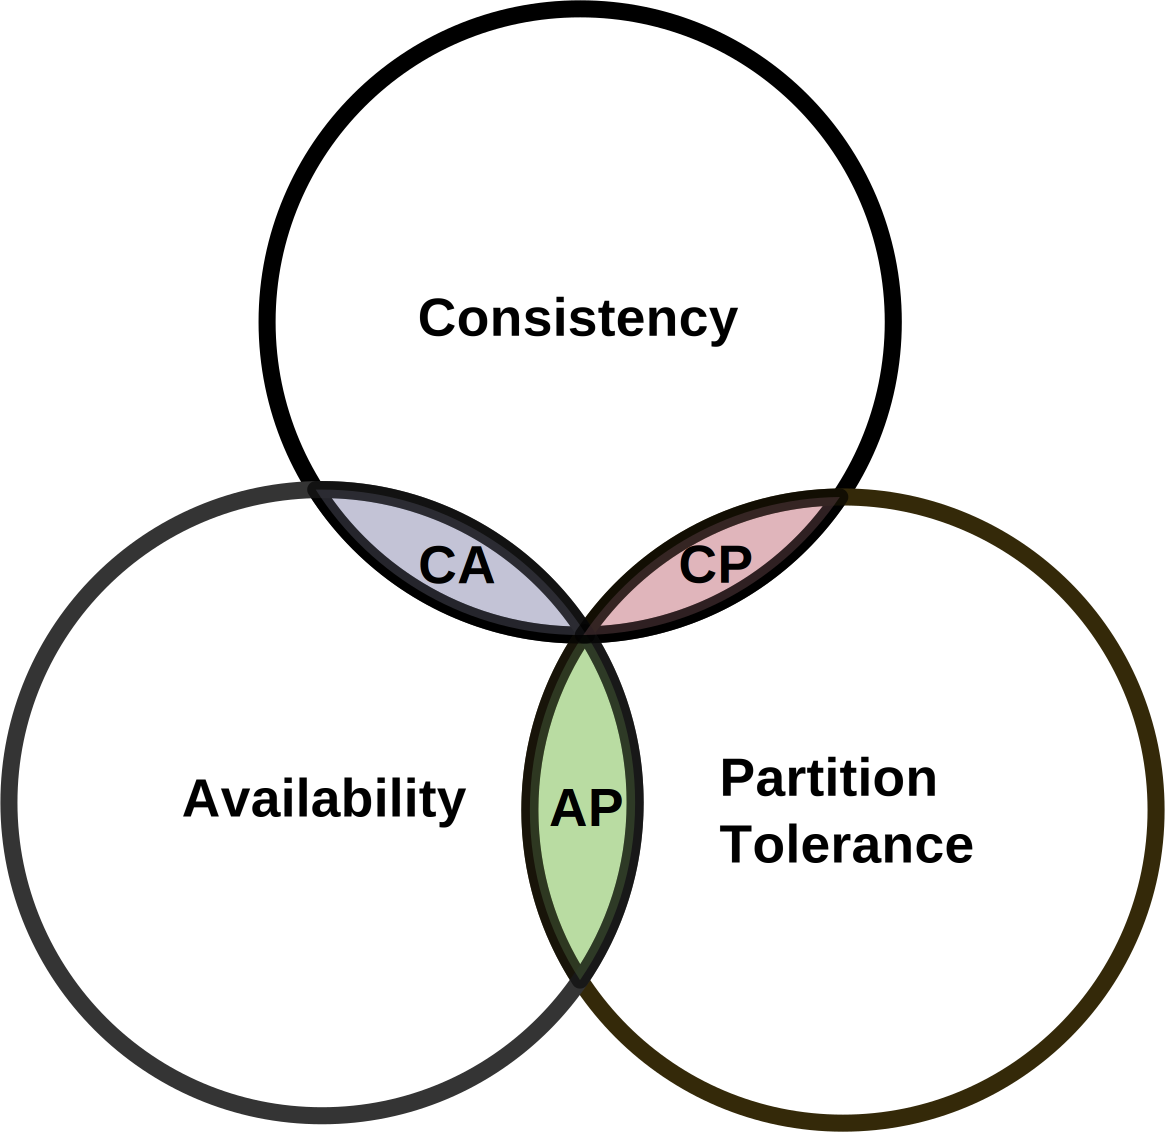
\includegraphics[width=0.5\textwidth]{cap.pdf}
  \caption{CAP theorem}
  \label{fig:cap}
\end{figure}

There are systems where total order of operations is not mandatory, these systems
choose to be partition tolerant. They are known as \textit{eventual consistent}
systems. A replica executes an operation without synchronizing its new state with
other replicas. This operation is sent asynchronously to the rest of replicas.
Every replica eventually applies the updates, without any guarantee about the
order in which these updates are applied. This approach establishes that data is
available even during network partitions. One of the problems of eventual
consistent systems is conflicting updates. Systems such Dynamo~\cite{dynamo}
allows to choose if clients should resolve conflicts or use simple approaches as
`last write wins'.

\acf{CRDT} provides a model based on simple mathematical properties that ensures
eventual consistency. \acs{CRDT}s do not require synchronization, since updates
are executed immediately. This property allows \acs{CRDT}s to be scalable and
fault-tolerant. In order to guarantee convergence in \acs{CRDT}s, data types
should follow the next properties:

A join semilattice~\cite{book:lattices} is a partial order $\leq_{v}$ equipped with a
least upper bound (LUB) $\sqcup_v$, defined as follows:

\begin{definition}{(Least Upper Bound (LUB))}
  $m = x \sqcup_v y$ is a Least Upper Bound of $\{x, y\}$ under $\leq_{v}$ \textit{iff}
  $x\leq_{v}m$ and $y\leq_{v}m$ and there is no $m'\leq_{v}m$ such that $x\leq_{v}m'$ and $y\leq_{v}m'$.
\end{definition}

It follows from the definition that $\sqcup_v$ is commutative: $x \sqcup_v y =_v y \sqcup_v x$; idempotent:
$x \sqcup_v x =_v x$; and associative: $(x \sqcup_v y) \sqcup_v z =_v x \sqcup_v (y \sqcup_v z)$.


\begin{definition}{(Join Semilattice)}
  An ordered set ${S, \leq_v}$ is a \textit{Join Semilattice} \textit{iff}
  $\forall x, y \in S, x \sqcup_v y$ exists.
\end{definition}

A \acs{CRDT} whose payload takes its values in a semilattice and where
\textbf{merge}$(x,y) = x \sqcup_v y$, converges towards the LUB of the initial
and updated values.

Given the described properties, \acs{CRDT}s are a good fit for highly scalable systems
such as Alcaudon aims to be. For contexts such as cluster membership or non-centralized
replication \acs{CRDT}s could be used in order to implement different Alcaudon sub-systems.

\subsection{Distributed system reliability}

Building distributed systems is not an easy task. In this subsection, different
failure scenarios that can happen in a distributed environment will be presented.

As proposed by ~\cite{GuideReliable}, it is possible to classify system error
causes as follows:
\begin{itemize}
\item \textit{Hardware failures}: These kind of failures are inevitable, since
  hardware has a life cycle and some components might fail or maintenance for
  components should be taken care of.
\item \textit{Software failures}: Software is becoming more and more complex.
  Software complexity errors such as coding errors, misguided software design,
  memory leaks or inadequate specifications are inevitable. There are countless
  examples of millionare losses, like when in 1999 NASA lost a Mars orbiter
  spacecraft because one team was working with Imperial units while another used
  metric units.
\item \textit{Complexity}: Developing software in distributed systems is
  complex. The notion of global state or order is fuzzy. Asynchronous
  communication is the norm. Regular developers are used to sequential
  computations, and getting familiarized to work within this environment is hard
  and can lead to bogus implementations. Luckily the use of formal verification
  is growing in the field, using tools such as TLA+~\cite{tla} by Lamport. The
  usage of these techniques helps to tackle the inherent complexity with strong
  foundations.
\item \textit{Lack of failure detectors}: Most distributed systems try to detect
  failure just by using timeouts. This measure is quite straightforward to
  implement and reason about. The main drawback is that these techniques are
  raw. Vogels ~\cite{vogels} proposes a refinement over plain timeouts for
  failure detection, using more meta-information about the environment where
  the distributed system is running; reasoning about operating system metrics,
  networking metrics and disseminated probes, failure detection can improve.
\item \textit{Hostile environments}: There has been enumerated some reliability
  threats, which distributed systems need to deal with. Those threats are in
  \textit{control}, meaning that the developers of the system should anticipate
  them. Designing the systems so they are ready to deal with the exposed
  problems. However those systems run in shared networks where security threats
  are a reality. It is a wide field and it is becoming more and more important
  to take all the possible measures to avoid security vulnerabilities.
\end{itemize}

As a final note about other problems, there are costs associated with
distributed programming; network latency, fault-tolerance mechanisms and
consensus can have impact in the throughput achieved by a system. In
~\cite{189908} a metric named Configuration that Outperforms a Single Thread
(COST), is proposed. It measures the number of cores needed to outperform a
single threaded implementation. In these experiments, there are many distributed
processing frameworks that don't perform properly when compared to single node
implementations. As a conclusion, there are scenarios where the costs associated
with distributed computing are higher than the gains.

Alcaudon's goal is to provide users a simple but powerful interface that enables
them to parallelize and distribute computations for unbounded datasets without all
the described problems.

\subsection{Actor Model}

To tackle all the complexity described in previous sections there is a
computation model that is well suited: the actor model.

The actor model provides a high level abstraction to deal with concurrent and
distributed systems. The theoretical model was developed by Carl Hewitt in
the seventies, but it was popularized by Erlang programming language~\cite{erlang}
developed by Ericsson.

It can be characterized as follows:
\begin{itemize}
\item Actors communicate via asynchronous messages
\item Actors manage their state
\item In the event of a message response they can:
  \begin{itemize}
  \item Create new child actors
  \item Send messages to another actors
  \item Stop actors (even themselves)
  \item Change their behavior for the next messages
  \end{itemize}
\end{itemize}

Since distributed systems communicate asynchronously, this model fits perfectly,
because, even in single node environments, all the computations are executed in
response to asynchronous messages. The fact that the shared state among actors
is minimal helps to tackle all the inherent complexities around concurrency.
Another interesting outcome from designing the systems using message passing is
that creating protocols comes naturally in this model. The ability to change
their behavior depending on the incoming messages makes easy to model finite
state machines that fit perfectly with protocol design.

There are many implementations available\FIXME{tag extraño en la referencia}~\cite{wikiactor}, but the more popular
and stable versions are the Erlang programming language and Akka. Both versions
have similar features, in fact, Akka is highly inspired by Erlang. Nevertheless
Akka is built on top of the \ac{JVM}, making it the most interesting implementation
available due to the vast ecosystem accessible around the \acs{JVM}.

Akka has some extensions to the actor model that make it quite interesting to
build distributed systems.
%
\begin{itemize}
\item Actor supervision: One interesting approach of actor based design is how
  to handle failures. Each actor has a supervisor that handles its life-cycle,
  exceptions included. With this supervision schema it is easier to isolate failure
  scenarios into specific actors instead of affecting the whole system. Each
  supervisor can define a strategy to apply when a child actor fails, i.e.
  restarting the actor or stopping it. This is highly beneficial because error
  handling logic is separated from business logic. These patterns resemble how
  ships are built, where the hull is compartmentalized into different watertight
  bulkheads. Therefore, if the hull is broken, the failure is limited to that
  bulkhead without compromising the ship stability. Alcaudon will benefit from
  this pattern to achieve fault-tolerant computations. One actor supervision
  tree can be found in figure~\ref{fig:supervision}.
\item Logical addresses: Each actor has a virtual address based on the actor
  system and its hierarchy. This helps providing location transparency, as
  actors can change their physical location and the framework will take care of
  routing messages to the new actor location.
\item Clustering: Support for distributed actors is provided, combined with
  logical addresses facilitates writing distributed applications.
\item Persistence: Akka supports actor state persistence. It is implemented as
  an append-only log. That technique is commonly used as transaction log in
  traditional databases, each change is appended to the transaction log. In case
  of a failure, those events are applied again to the in memory database
  buffers. To avoid long recovery times, snapshots from memory are taken
  regularly so the recovery process just needs to re-apply changes from that
  point. Akka persistence is implemented as described. This feature fits very
  well to mantain Alcaudon persistent state of computations, since computations
  can be defined as actors.
\end{itemize}

\begin{figure}[!h]
\begin{center}
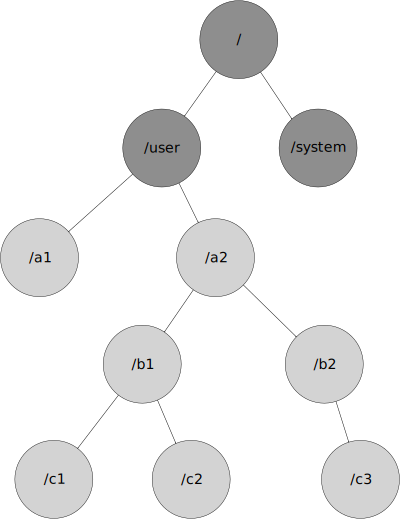
\includegraphics[width=0.5\textwidth]{supervision.pdf}
\caption{Actor supervision tree}
\label{fig:supervision}
\end{center}
\end{figure}

In conclusion, the actor model is a good computational model to base Alcaudon
on. It has properties that allows tackling all the presented difficulties around
writing distributed systems properly.

\section{Job scheduling}

Computations in distributed data processing clusters are expressed as a
dataflows. They can be considered as a direct acyclic graph (DAG) as the one in
Figure~\ref{fig:dataflow}.

\begin{figure}[h!]
\begin{center}
\includegraphics[width=0.6\textwidth]{dataflow.png}
\caption{Dataflow}
\label{fig:dataflow}
\end{center}
\end{figure}

One open problem in the construction of distributed data processing systems is
how to place those computations represented as a \acs{DAG}, given a set of computing
nodes. This problem is known as the flexible Job-shop scheduling problem and it
has been widely studied during the last 60 years. One graphical example for $3$
jobs to be scheduled along $3$ machines can be seen in Figure~\ref{fig:jssp}.
As defined in~\cite{jobshop2}:

\begin{definition}
In the flow shop scheduling problem we have a set of $n$ jobs that must be
processed on a given set of $m$ machines that are located in a fixed order. Each
job $j$ consists of a sequence of $m$ operations, where the $i$-th operation
must be processed during $p_{ij} \in \Z^{+}$ Time units without interruption on
the $i$-th machine. A feasible schedule is one in which each operation is
scheduled only after all operations preceding it in its job have been completed,
and each machine processes at most one operation at a time. A natural
generalization of the flow shop problem is to not require jobs to be processed
on all machines, i.e., a job still requests the machines in compliance with
their fixed order but may skip some of them. We will refer to this more general
version as generalized flow shops or flow shops with jumps. Generalized flow
shop (and thus flow shop) scheduling is a special case of the acyclic job shop
scheduling, which only requires that within each job all operations are
performed on different machines, which in turn is a special case of the general
job shop scheduling, where each job may have many operations on a single
machine. For any given schedule, let $C_j$ be the completion time of the last
operation of job $j$. We consider the natural and typically considered
objectives of minimizing the makespan, $C_{max} = max_j C_j$ , and the
\textit{sum of weighted completion times}, $\sum w_jC_j$ , where $w_j$ are
positive integers. The goal is to find a feasible schedule which minimizes the
considered objective function.
\end{definition}

\begin{figure}
\begin{center}
\includegraphics[width=0.6\textwidth]{jssp.png}
\caption{ A Gantt-Chart representation of a solution for a $3m \times 3j$ job scheduling problem~\cite{geneticbook}}
\label{fig:jssp}
\end{center}
\end{figure}

Computing an optimal solution for this problem is a well known NP-hard
problem~\cite{nphard}. Given this fact, all the proposed algorithms to solve this
problem are approximation algorithms. Some of the techniques used are listed
below:

\begin{itemize}
\item Algorithms based on priority rules and active schedule generation
\item \textit{Shifting bottleneck}
\item Simulated annealing
\item Tabu search
\item Genetic algorithms
\end{itemize}

Alcaudon will use an state-of-the-art scheduling framework,
Firmament~\cite{firmament}, in order to solve this problem.

\section{Library design}

Humans have been using abstraction since the very beginnings of their existence.
The reality around is too complex to understand every detail of it. Thus,
abstraction is a really excellent tool to extract just the relevant facts about
the studied phenomenons. Computer Science, Software Engineering and Electrical
Engineering combine different abstractions in order to to build complex systems
in a manageable way.
Computer Science provides the tools whose roots are based on mathematical
foundations such as automaton theory, lambda calculus, language design, data
structures, etc.
Using those ideas, software engineering can be seen as the bridge between
hardware and computer science. It builds abstractions based on both worlds such
as operating systems, that hides the details of specific hardware and exposes an
uniform interface. And the list goes on.

The main goal of abstractions is to
provide ways to reason about different problems with a limited scope.
As it has been exposed, providing tools that hide all the complexities is key to
build more complex systems. One of the main goals of the field since the late
60s has been to build reusable software~\cite{reuse}. There have been many
advances in code reuse, from libraries and frameworks that are used to build
software on top them, to \acf{SaaS}. SaaS exposes public \ac{HTTP}
\ac{API} as the entry point to their functionality. This category of software reuse
can be the end of the spectrum, since the client just has knowledge about
the exposed interface and does not know anything about the underlying parts of the
system.

\begin{figure}[!h]
\begin{center}
\includegraphics[width=0.8\textwidth]{serverless.png}
\caption{Serverless architecture example~\cite{awsserverless}}
\label{fig:serverless}
\end{center}
\end{figure}

One recent trend in industry is serverless architecture like the one shown in
Figure~\ref{fig:serverless}. This programming model has foundations in reactive
programming, and it is based on providing code to produce computation results as
response to changes or events. In this paradigm it is just needed to provide
code implementing certain interface~\ref{code:lambdalisting} to handle events,
such as database changes, and the system will take care of deploy and run those
pieces together. As it can be observed, abstraction is going upwards and
programmers just need to take care of writing business logic and building
robust programs.

\begin{lstlisting}[language=java, frame=trBL, label=code:lambdalisting, float=ht, caption = {AWS Lambda Interface}]
  public interface RequestStreamHandler {
    public void handleRequest(InputStream inputStream, OutputStream outputStream, Context context)
    throws IOException
  }
\end{lstlisting}

Alcaudon philosophy is similar to the serverless architecture. The goal is to
provide abstractions around unbounded datasets so programmers just take care of
defining their computations and dependencies. Alcaudon will provide a simple
interface so the details to know about the system are minimized.

% Local Variables:
% ispell-local-dictionary: "american"
% End:

\chapter{Methodology}
\label{chap:methodology}

\drop{T}{he} software methodology used to develop this project will be described in this
chapter. Agile methodologies have been used to drive Alcaudon's development.

Agile methodologies help organizing software development life cycle. They are
focused on iterative development and adaptability. The term was coined during
the early 2000s in the \textit{Agile Manifesto}\cite{manifesto}. The manifesto
has this set of principles:

\begin{itemize}
\item Individuals and interactions over processes and tools
\item Working software over comprehensive documentation
\item Customer collaboration over contract negotiation
\item Responding to change over following a plan
\end{itemize}


\begin{figure}
  \centering
  \includegraphics[width=0.8\textwidth]{agile.jpg}
  \caption{Waterfall vs Agile Methodologies\cite{waterfall}}
  \label{fig:waterfall}
\end{figure}

The main goal of these methodologies is to improve communications between all
the stakeholders in a project. This focus on continuous communications reduces
risks and provides value since the very beginning of the project. One of the
outcomes of this iterative open process is a reduction in the costs of the
changes. This differs totally from rigid methodologies such as waterfall where
the customer is taken apart from the project until the very end, skyrocketing
the costs of change as shown in Figure~\ref{fig:waterfall}.

Agile methodologies have become popular during the last 10 years, therefore there
are many agile frameworks that follow the previously enumerated principles. The
most popular ones are:
\begin{itemize}
\item SCRUM\cite{scrum}: Framework that allows teams to develop complex
  adaptive software delivering value as soon as possible.
\item eXtreme Programming\cite{xp}: Lightweight methodology for small-medium
  sized software development teams in scenarios where requirements change often
  or are vague.
\item Kanban\cite{kanban}: Inspired by the work of Toyota during the 1940s to improve
  factory resource utilization, this lightweight methodology also minimizes the processes
  around development. It is focused on having a set of features to be done and delivering
  them as soon as possible. It is a good fit for startup teams.
\end{itemize}

Since Alcaudon's requirements were not clear from the start, agile methodologies
provided the optimal framework. In particular, \acf{XP} was chosen
due to the team's small size and the expected requirement changes.

\section{eXtreme Programming}

\begin{figure}
  \centering
  \includegraphics[width=0.6\textwidth]{xp.png}
  \caption{Extreme Programming feedback diagram\cite{xp}}
  \label{fig:xp}
\end{figure}

This methodology proposes a feedback/release cycle as shown in Figure~\ref{fig:xp} and a set of
practices\cite{xp}:

\begin{enumerate}
\item \textit{The planning game}: The scope, priority and date of releases
  should be agreed between business and technical team, adapting them in the
  face of unplanned events. Neither business nor technical parties involved have
  more weight than the other when planning next releases. This is why
  communication is one of the key principles in this methodology. In Alcaudon
  the business team was represented by the advisor, \textit{David Villa Alises},
  and the technical team by the author.
\item Small releases: Every release should be as small as possible providing the
  maximum business value. Alcaudon was released continuously, meaning that it
  has adopted Continuous Deployment\cite{cd} techniques. With every commit
  pushed to the master branch, Travis CI\footnote{https://travis-ci.org/}
  launched a continuous delivery pipeline that run tests, built and published
  an usable version of Alcaudon as docker containers and a snapshot version of
  the libraries to a repository. This practice allows Alcaudon's process to
  bring value as soon as possible. Moreover, it reduces risks, thus contributing
  to build a more efficient and robust system.
\item \textit{Metaphor}: A common language between different participants in the
  project should be used. This makes communication easier and therefore
  misunderstandings are reduced.
\item Simple design: As defined by\cite{xp}, a simple design follows these rules:
  \begin{enumerate}
  \item All tests pass.
  \item There is no duplicated logic.
  \item States every intention important to the programmers.
  \item Has the fewest possible classes, methods and functions.
  \end{enumerate}
  Alcaudon follows these principles. Consequently, the risks associated to
  changes are minimized.
\item Testing: In \acs{XP} there is a strong bias towards writing tests for all the
  created features, both unit and functional tests. This practice creates
  a stronger confidence in programmers when they need to change their code.
  Alcaudon has been tested broadly, using unit, integration and property based
  testing. Having a good testing coverage has helped to keep developing the
  system with confidence in its correctness, since this project can not be
  easily tested manually.
\item Refactoring: Given the previous principle of \textit{simple design},
  continuous design refinement via refactoring is a key concept in \acs{XP}.
  Refactoring helps to keep control of complexity iterating over software
  design, reducing risks in future changes. During the development of this
  project, there have been some refactors that improved the design of certain
  modules. Following this principle has been crucial to improve the system's
  architecture.
\item Pair programming: In this methodology there is a preference towards programming
  in pairs. Different points of view can improve the final design and spot
  possible failures that otherwise would have taken longer to detect. This
  principle does not apply to Alcaudon since it is an individual project.
\item Continuous Integration: Code should be integrated and tested every few
  hours. This practice helps to avoid working too long in a big feature, making
  it harder to integrate later. Again, \acs{XP} is favoring risk reduction with this
  set of practices. As described before, Alcaudon uses Travis CI as continuous
  integration server, for every commit to master the project is built and
  tested.
\item On-site customer: \acs{XP} accentuates the importance of communications. A
  domain expert, i.e. an user, should be available to answer questions about the
  business and set small scale priorities. Having this person accessible, saves
  time when developers are not familiar with some details about the domain, therefore
  reducing risks.
\item Coding standards: Every project should have coding standards so the
  differences in style among the code written by the team are minimized. An
  example could be a code linter, so if there is a deviation in the defined
  style the programmer will be warned. There are more sophisticated tools to
  define standards, such as code quality measurements tools. These metrics can
  be added in the continuous integration pipeline. if the added code does not
  comply with them, the build is marked as failed. This project uses a code
  linter and advanced compiler warnings (such as unused code, deprecated APIs,
  etc), therefore the coding style is uniform.
\end{enumerate}

\subsection{eXtreme Programming applied to this project}

This section describes the different releases done during the development of
Alcaudon. As it has been stated before, Continuous Deployment has been
implemented, so there has been a production ready release after every code
change. For simplicity this section will describe release cycles with blocks of
features.

\subsubsection{Release 1: State of the art analysis}
\begin{itemize}
\item \textit{Agreed goal}: Distributed data processing systems state-of-the-art analysis.
  \item \textit{Deliverable}: Document describing existing solutions in the
    distributed data processing space as well as recent developments from
    different related conferences such as VLDB, SIGMOD and OSDI.
\end{itemize}

\subsubsection{Release 2: Technology selection}
\begin{itemize}
\item \textit{Agreed goal}: Given the findings from the previous release,
  investigate suitable technologies to implement a distributed data processing
  system.
\item \textit{Deliverable}: After some investigation and tests two languages
  were chosen, Erlang and Scala. Both implement the actor model. Erlang has been
  proven to be production ready, but according to TIOBE\cite{tiobe} its usage is
  not ample. On the other hand, Scala seems to be quite popular among the data
  processing community. After some discussion with business stakeholders, Scala
  was chosen due to its inter-operability with Java and notoriety among
  developers.
\end{itemize}

\subsubsection{Release 3: Computation, timer, source and sink API definitions}
\begin{itemize}
\item \textit{Agreed goal}: Define the public interface that customers will use
  to implement their computations and timers as well as sources and sinks.
\item \textit{Deliverable}: During this release cycle, communication between the
  different participants in the project was quite productive. A first proposal
  was sent to the domain expert, the advisor in this project. This first version
  did not take into account certain details that were key to the project. Given
  the early feedback, it was possible to react quickly and present a new
  computation API that contained less details about the implementation,
  providing a better abstraction.
\end{itemize}

\subsubsection{Release 4: Dataflow builder development}
\begin{itemize}
\item \textit{Agreed goal}: Develop a first dataflow builder version where the
  user can define a dataflow topology.
\item \textit{Deliverable}: During this release an usable dataflow builder was
  delivered. Alcaudon users were able to build their own computation topologies.
  This allowed to start testing how usable the interface was and with the given
  feedback improve the initial designs.
\end{itemize}

\subsubsection{Release 5: First computation execution engine version development}
\begin{itemize}
\item \textit{Agreed goal}: Implement the first version for the computation
  execution engine.
\item \textit{Deliverable}: Since Dataflow builder was developed during the previous
  release, the next natural step was to implement the computation executor.
  During this release a simplified engine version was released, making possible
  to test simple computations.
\end{itemize}

\subsubsection{Release 6: Computation execution guarantees development}
\begin{itemize}
\item \textit{Agreed goal}: Implement means to provide fault-tolerant computation executions.
\item \textit{Deliverable}: One of the Alcaudon goals is to be fault-tolerant.
  The outcome of this release cycle was fully tested computation engine that
  complies with the fault-tolerant agreed requirements.
\end{itemize}

\subsubsection{Release 7: Timer execution engine development}
\begin{itemize}
\item \textit{Agreed goal}: Implement fixed and watermark based timers.
\item \textit{Deliverable}: Alcaudon works with unbounded data-sets, hence a way
  to emit partial results should be provided. In this release, fixed timers and watermark
  timers were released. Watermarks were developed using \acs{CRDT}s.
\end{itemize}

\subsubsection{Release 8: Generic serialization library development}
\begin{itemize}
\item \textit{Agreed goal}: Develop generic serialization library for Algebraic
  Data Types.
\item \textit{Deliverable}: Data travels around Alcaudon as an array of bytes.
  There are many serialization formats to transform high level entities to
  binary data. However, for simplicity, a generic serialization library has been
  developed. This library is able to, given an Algebraic Data Type, create a
  serializer/de-serializer using scala implicit induction during compile time.
\end{itemize}

\subsubsection{Release 9: Stream entity implementation}
\begin{itemize}
\item \textit{Agreed goal}: Implement a Stream representation so data can be
  published and consumed from it. Published data should be durable.
\item \textit{Deliverable}: Since computations subscribe to streams, in this release a
  durable stream representation was implemented. This allows consumers and publishers to
  consume and publish stream records. During this release, given the changes
  that appeared during the design of the stream entity, some refactors in the
  computation execution engine were done.
\end{itemize}

\subsubsection{Release 10: Library manager implementation}
\begin{itemize}
\item \textit{Agreed goal}: Implement a subsystem that enables dynamic load of
  arbitrary user code into remote Alcaudon workers.
\item \textit{Deliverable}: A module to load arbitrary user code was developed.
  It is backed by a cloud object storage\footnote{https://aws.amazon.com/s3/},
  and allows dynamic load of user code.
\end{itemize}

\subsubsection{Release 11: Distributed architecture design}
\begin{itemize}
\item \textit{Agreed goal}: Design a resilient distributed architecture that
  allows remote work distribution for the system.
\item \textit{Deliverable}: During this release some requirement changes were brought
  by the business side due to a bug in the stream implementation. Given the urgency
  of those changes, just a partial design was done.
\end{itemize}

\subsubsection{Release 12: Distributed architecture implementation}
\begin{itemize}
\item \textit{Agreed goal}: Finish the first design for the distributed
  architecture and implement a prototype.
\item \textit{Deliverable}: In this release, a first version for the distributed
  architecture was developed. The idea was to keep developing during the next
  release cycles.
\end{itemize}

\subsubsection{Release 13: Implement job scheduling policy}
\begin{itemize}
\item \textit{Agreed goal}: Implement computation scheduling to distribute the
  dataflow topology in the most optimal possible configuration.
\item \textit{Deliverable}: Due to the time constraints, during this release it
  was decided to use available tools to solve the flexible job-shop scheduling
  problem. In this case, a state-of-the-art flexible scheduler was used\cite{firmament}.
\end{itemize}

\subsubsection{Release 14: Implement tools that allow monitoring the system}
\begin{itemize}
\item \textit{Agreed goal}: Implement tools or adopt external tools that allow
  observing the behavior of the system.
\item \textit{Deliverable}: After some investigation it was agreed to used both
  an external system to facilitate observability, Prometheus, and implement some
  tools to track how the system is performing.
\end{itemize}

\subsubsection{Release 15: implement some sources and sinks}
\begin{itemize}
\item \textit{Agreed goal}: Provide some default implementations of sources and
  sinks, such as TCP sockets or Twitter streaming api.
\item \textit{Deliverable}: During this release the agreed goals were implemented. Given
  that the system needed some improvements, this latest release was used also to refactor
  some modules of the system to give them more reliability.
\end{itemize}

\section{Development technologies}

There are many technologies available to develop information systems. Different
paradigms, different environments, etc. For Alcaudon, working with the \acs{JVM}
was the perfect match. It is one of the most advanced language virtual machines
in the market, with outstanding implementations such as
OpenJDK\footnote{http://openjdk.java.net/} or
Zing\footnote{https://www.azul.com/products/zing/virtual-machine/}. The
available ecosystem of tools and libraries covers many domains. There are
multiple implementations for the state-of-the-art data structures used in this
project, such as cuckoo filters\cite{cuckoo}. Another reason to choose the \acs{JVM}
was the inter-operability between different languages such as Scala and Java.
Scala has been chosen as the principal programming language. It is an hybrid
language that allows programmers to use functional and object oriented
programming paradigms. The compelling aspect of this design is that it allows
the combination of the best of both worlds. It provides tools to work with
functional constructs such as monadic composition or use more object oriented
tools such as traits.

In the database space, \textit{Cassandra} has been chosen as the principal data store due
to its design with high availability and scalability in mind. This choice
provide good grounds to guarantee data durability within the system. For storing
time series data, \textit{Prometheus} has been chosen due to its high scalability and
performance querying historic data.

Another tool used in the development Alcaudon has been \textit{TravisCI}, a
cloud continuous integration service. Using a service that is fully integrated
with git facilitated the set-up of the continuous deployment pipeline easier.

\section{Tools}

In this section the tools used to develop Alcuadon will be presented. 

\subsection{Hardware}

The only physical hardware used to develop this project has been a laptop. For
deploying the system, Amazon Web Services has been used. All the incurring costs
for testing have been assumed by the author of this project.

\begin{itemize}
  \item Dell XPS 13 with Intel\textregistered Core\texttrademark i5 2.5GHz
    processor 8GB RAM DDR3 and 128GB SSD hard drive.
  \item Amazon Web Services provided servers with different specifications.
\end{itemize}

\subsection{Software}

\begin{itemize}
  \item Operating Systems
    \begin{itemize}
        \item Debian 8 Jessie\footnote{https://www.debian.org/index.es.html}.
          Operating system used to develop the system and the documentation.
        \item CoreOS\footnote{https://www.coreos.com/}. Minimal linux operating
          system that supports container systems out of the box. Used to deploy
          Alcaudon.
    \end{itemize}

  \item Languages
    \begin{itemize}
      \item Scala\footnote{https://www.scala-lang.org/}. Hybrid Functional and
        Object Oriented programming language used to develop the system.
      \item \LaTeX{}\footnote{https://www.latex-project.org/}. Language used to
        write this document.
    \end{itemize}

  \item Frameworks, libraries and databases
    \begin{itemize}
      \item Akka\footnote{https://akka.io}. Toolkit to develop actor based
        systems. Most of the system relies on the actor model. The following
        extensions have been used:
        \begin{itemize}
        \item akka-cluster
        \item akka-persistence
        \item akka-distributed-data
        \end{itemize}
      \item Shapeless\footnote{https://github.com/milessabin/shapeless}. Generic
        programming for Scala used to develop generic serializers.
      \item Apache Cassandra\footnote{http://cassandra.apache.org/}. Open source
        database aimed for scalability.
      \item Scala Graph\footnote{http://www.scala-graph.org/}. Graph data
        structure implementation for Scala.
      \item
        CuckooFilter4j\footnote{https://github.com/MGunlogson/CuckooFilter4J}.
        High performance Java implementation of a Cuckoo filter.
      \item ScalaCheck\footnote{https://www.scalacheck.org/}. Property based
        testing library for Scala.
      \item ScalaTest\footnote{http://www.scalatest.org/}. Testing framework for
        Scala.
      \item Kryo\footnote{https://github.com/EsotericSoftware/kryo}. Fast efficient serialization
        framework for the JVM.
      \item Prometheus\footnote{https://prometheus.io/}. Open
        source time series database used for monitoring.
      \item Firmament\footnote{http://firmament.io/}. Flexible cluster scheduler.
    \end{itemize}

  \item Tools
    \begin{itemize}
      \item sbt\footnote{http://www.scala-sbt.org/}. Build tool for Scala.
      \item Emacs \footnote{https://atom.io/}. Text editor used to program the system.
      \item Git\footnote{https://git-scm.com/}. Distributed version control system.
      \item TravisCI\footnote{https://www.travis-ci.org/}. Cloud continuous integration service.
      \item Docker\footnote{https://www.docker.com/}. Linux container runtime.
      \item Grafana\footnote{https://grafana.com/}. Open platform for analytics and monitoring.
    \end{itemize}

\end{itemize}

\chapter{Architecture}
\label{chapter:architecture}

Alcaudon's architecture will be described in this chapter following a top-down
approach. Firstly, a general description of the different components of the system
will be explained. Finally, each of the components will be described more thoroughly.

\subsection{General description}

Alcaudon's platform is composed by 3 main units.

\begin{itemize}
\item \textbf{Alcaudon library}: This is the main interface between users
  and the system. In order to use Alcaudon it is necessary to have access to a
  cluster with a coordinator and computing nodes. This interface is provided as
  a library containing the tools to build dataflows, the interfaces to implement
  user defined stream computations and the tools to connect with a particular
  cluster. Since the computations are potentially infinite, the operations
  performed against the cluster are asynchronous, returning an id associated
  with the created operation.
\item \textbf{Coordinator node}: This is the main component of the system. It
  coordinates the life cycle of the different components of the cluster such as
  the computing nodes. It is also responsible of performing the scheduling of
  the user defined dataflows given the resources provided by the computing
  nodes. Finally, it is the interface between the cluster and the users, where
  they deploy their dataflow topologies.

\item \textbf{Computing nodes}: These nodes are in charge of executing the
  actual computations provided by Alcaudon's users. These nodes take care of
  storing intermediate results published to streams. They register dynamically
  to the cluster contacting the coordinator node. A deployment can be composed
  from one computing node up to thousands, as needed. Each of these nodes
  provides certain resources to the system, known as \textit{computation slots}.
  The number of slots is configurable, but they correlate with the number of
  available CPU's in the underlying hardware.
\end{itemize}

A high level overview of the system can be seen in
figure~\ref{fig:architecture}. The majority of the parts of the system have been
modeled as Actors. As it was stated previously it is a very good fit for this
kind of applications. Where possible, object oriented design patterns\cite{gof}
such as \textbf{builder} or \textbf{factory} have been used. However, functional
programming constructs such as monads\cite{monads}, type
classes\cite{typeclasses} or Algebraic Data Types have been used more widely.

Once the different parts of the system have been presented, they will be
inspected in detail.

\begin{figure}[!h]
  \centering
  \includegraphics[width=0.9\textwidth]{architecture.pdf}
  \caption{Alcaudon architecture schema}
  \label{fig:architecture}
\end{figure}

\newpage
\subsection{Alcaudon library}

In the first place, the user facing interface will be presented in detail. In order
to create a streaming data processing pipeline, or dataflow topology as it has
been defined during all this document, users should provide their business
logic. To achieve this goal, Alcaudon provides certain interfaces so users
just need to care about their code. These interfaces are available as a library
that can be found at at Sonatype OSSRH \footnote{http://central.sonatype.org/pages/ossrh-guide.html}.

\begin{figure}[!h]
  \begin{center}
  \includegraphics[width=0.6\textwidth]{client.pdf}
  \caption{Alcaudon library}
  \label{fig:library}
  \end{center}
\end{figure}

This library is composed of three modules as it is shown in figure~\ref{fig:library}:

\begin{itemize}
\item Computation API's: Interface that users should implement in order to
  create computations.
\item Dataflow builder: This component is used to build dataflow topologies and
  later on submit the to the cluster coordinator.
\item Cluster client: Communication layer between clients and Alcaudon clusters.
  It handles all the operations needed to submit custom code to the cluster as well
  as the stream processing pipeline definition.
\end{itemize}

\subsubsection{Computation API's}

\begin{figure}[!h]
  \begin{center}
  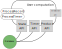
\includegraphics[width=0.5\textwidth]{libraryApi.pdf}
  \caption{Alcaudon computation API's}
  \label{fig:apis}
  \end{center}
\end{figure}

As explained before, in order to create custom computations to process unbounded
data-sets in Alcaudon, it is necessary to implement an interface. The interface
is listed in~\ref{code:computation}. This interface gives access to the
abstractions provided by the system as represented in figure~\ref{fig:apis}. As
it can be observed, there are two methods to be implemented;
\lstinline[columns=fixed]{def processRecord(record: Record): Unit} and \lstinline[columns=fixed]{def processTimer(timer: Timer): Unit}.

\begin{lstlisting}[language=scala, frame=trBL, label=code:computation, float=ht, caption = {Computation API's}]
trait Computation
    extends ProduceAPI
    with TimerAPI
    with StateAPI
    with SerializationAPI
    with RuntimeContext {
  ...
  def processRecord(record: Record): Unit
  def processTimer(timer: Timer): Unit
  ...
}
\end{lstlisting}

These methods represent the main entry point into user code, hooked in reaction to
record receipt and timers expiration. These constitute the application logic.
Within the execution of these methods, Alcaudon provides different functions to
work with persistent state, publish new records to streams, set timers or
serialize arbitrary data types. Those auxiliary API's are listed
in~\ref{code:auxiliaryComputations}. In Alcaudon, each computation can subscribe to
multiple sources represented as streams. Data travels in its simplest form,
as an array of bytes.

\begin{figure}[!h]
  \begin{center}
    
\includegraphics[width=0.5\textwidth]{keypartitioning.pdf}
    \caption{Alcaudon record key assignment}
    \label{fig:keypartitioning}
  \end{center}
\end{figure}

However, for each stream subscription users should provide
a key extraction function, this process can be shown in figure
~\ref{fig:keypartitioning}. Having a key per record allows the implementation of
parallelization strategies such as key partitioning. Therefor, every record
emitted by one of the subscribed sources, an instance of the class
\lstinline[columns=fixed]{Record} listed in ~\ref{code:records} will be
injected with the call to \lstinline[columns=fixed]{processRecord}.

\begin{lstlisting}[language=scala, frame=trBL, label=code:records, float=ht, caption = {Record classes}]
case class RawRecord(value: Array[Byte], timestamp: Long) {
  val id = UUID.randomUUID().toString
}
case class Record(key: String, rawRecord: RawRecord) {
  val value = rawRecord.value
  val timestamp = rawRecord.timestamp
  val id = UUID.randomUUID().toString
}
\end{lstlisting}

Timers are the other possible trigger for user defined code execution. In
Alcaudon there are three types of timers:

\begin{itemize}
\item \textit{Fixed timers}: This kind of timers are triggered once at a
  specific wall time.
\item \textit{Recurrent fixed timers}: This timer is just like the previous
  timers, however it is executed recurrently. I.E., every five minutes.
\item \textit{Watermark timers}: This timer try to estimate the point where all
  the events up to certain window have been consumed by the system and execute
  then. The mechanism and algorithm used to implement them will be explained
  later.
\end{itemize}

When a timer is executed it has as a parameter an instance of the class Timer
listed in ~\ref{code:timers}. This constructs are key to the domain of unbounded
data-sets due to its very nature. A mean to emit partial results is needed, so
this is the mechanism provided by Alcaudon to emit results.

\begin{lstlisting}[language=scala, frame=trBL, label=code:timers, float=ht, caption = {Timer class}]
  case class Timer(tag: String, timestamp: Long)
\end{lstlisting}

\subsubsection{Dataflow builder}

Once the computations are implemented, users need a way to build the dataflow topologies.
To achieve this goal, the system provides a dataflow builder. It is based on a very well
known design pattern, the builder pattern. Using this class, users are able to define
the dependencies among the main entities in the system. These main entities are:

\begin{itemize}
  \item \textit{Sources}: 
  \item \textit{Computations}:
  \item \textit{Streams}:
  \item \textit{Sinks}:
\end{itemize}


MOVE 
\begin{lstlisting}[language=scala, frame=trBL, label=code:auxiliaryComputations, float=ht, caption = {Computation API's}]
trait ProduceAPI { environment: RuntimeContext =>
  protected def produceRecord(record: RawRecord, stream: String): Unit =
}

trait TimerAPI { environment: RuntimeContext =>
  protected def setTimer(timer: Timer): Unit
}

trait StateAPI { environment: RuntimeContext =>
  protected def set(key: String, value: Array[Byte]): Unit
  protected def get(key: String): Array[Byte]
}

trait SerializationAPI {
  def serialize[T](data: T)(implicit ti: TypeInfo[T]): Array[Byte]
  def deserialize[T](binary: Array[Byte])(implicit ti: TypeInfo[T]): T
}
\end{lstlisting}

\chapter{Results}

In this chapter, attained results during the development of this project will be
presented. First, a series of benchmarks have been used in order to
exercise key Alcaudon modules and measure how the system behaves. To conclude,
a summary of accomplished objectives is presented.

\section{Benchmarks}

Alcaudon has been tested thoroughly, both using traditional testing techniques
as well as more state-of-the-art techniques such as property based testing.
These tests can guarantee correctness in terms of behavior, but they do not
measure system correctness in terms of performance goals. Even though Alcaudon
has been designed carefully, using the adequate data structures and taking
care of performance, empiric results are needed. It is known that creating
accurate benchmarks is complex~\cite{benchbias}, there are many factors
that can lead to misleading results. Presented benchmarks are implemented using
JMH\footnote{http://openjdk.java.net/projects/code-tools/jmh/} trying to be as
accurate as possible.

\subsection{Computation execution benchmark}

This benchmark measures the number of computations per second that Alcaundon can
handle.

\FIXME{TODO -> figure}

\subsection{Stream benchmark}

This benchmark measures the number of records that a stream can handle.

\FIXME{TODO -> figure}

\subsection{Record router benchmark}

This benchmark measures the number of records that a router can route.

\FIXME{TODO -> figure}

\section{Accomplished objectives}

During the development of this project, all objectives defined at the beginning
of this document have been accomplished. Alcaudon provides all the necessary
tools to deploy distributed stream data processing pipelines. It attains this
objective by supplying an abstract model, the Computation \acs{API}, that users
implement, leveraging the all the complexities around fault-tolerant distributed
models to Alcaudon.

Regarding specific objectives, these have been accomplished as well:
%
\begin{itemize}
\item Alcaudon provides an abstraction in order to create distributed
  computations; computation \acs{API} alongside the dataflow builder.
\item The system provides exactly-once processing semantics, using at-least once
  delivery in combination with idempotent record processing. In order to achieve
  idempotence, state-of-the-art probabilistic data structures have been used as
  well as persistent actors to guarantee persistent state durability.
\item The system provides watermark based timers in order to work with
  out-of-order data. The implementation of this subsystem uses state-of-the-art
  coordination-free distributed data types in order to replicate knowledge about
  time event evolution inside the system.
\item Dataflow \acs{DAG}s are scheduled into available compute nodes using an
  state-of-the-art flexible cluster scheduler~\cite{firmament}. Different scheduling
  policies can be configured depending on the needs, where the default choice is
  biased towards co-location.
\item Several sources and sinks are provided by default such as Twitter streaming
  API, TCP Sockets or Apache Kafka. However it is possible to implement new ones
  just extending SourceFn and SinkFN interfaces.
\item Alcaudon provides an elastic distributed implementation where compute
  nodes can join the cluster in the events of burst of load. The system has been
  designed in order to be resilient and fault-tolerant. The actor model has
  helped a lot in terms of resilience due to is supervision mechanism that
  allows to isolate failure.
\item Alcaudon provides different metrics about the state of the system. It has been
  integrated with industry proven technologies in the space of monitoring such as
  Prometheus and Graphana. Using these tools it is possible to create a rich set
  of alerts and dashboards giving a good overview of how the different components
  of Alcaudon perform.
\item Alongside the previously presented results, Alcaudon is distributed using Docker
  containers and its library is available in SonaType repository. This makes almost
  trivial to deploy a full-featured Alcaudon cluster.
\end{itemize}

\section{Future work}

Given that Alcaudon has been designed in a modular way and it has many automatic
tests, including new features should effortless. In this section some future work
that could be done to the platform is presented.

\begin{itemize}
\item Improve system performance avoiding object allocations in certain
  sensitive parts of the system such as the Streams. High allocation rate
  usually hurts managed systems performance due to garbage collection. Some
  systems such as Netty\footnote{https://netty.io/} use pre-allocated memory buffers
  in order to avoid heap allocations as much as possible. This approach could be
  explored in order to improve Alcaudon performance.
\item Implement a machine learning algorithm in order to select a scheduling policy
  based on similar already run dataflow pipelines, improving the overall performance.
\item Implement a fully functional programming interface on top of the
  computation API in order to offer a more expressive API to the users.
  Providing \textit{combinators} such as map, groupBy, filter, etc.
\item Alcaudon watermark algorithm is just a minimal version. Used heuristic
  could be improved and it would be interesting to test different machine
  learning algorithms in order to predict watermarks. Another interesting
  approach to the problem that watermarks solve is to use virtual tables as
  Apache Kafka Streaming does~\cite{kafkastreams}.
\end{itemize}


\appendix
\appendixtitle
\chapter{Alcaudon configuration}

\begin{lstlisting}
akka {
  loglevel = "INFO"
  stdout-loglevel = "INFO"

  persistence {
    journal.plugin = "cassandra-journal"
    snapshot-store.plugin = "cassandra-snapshot-store"
  }

  actor {

  provider = "akka.cluster.ClusterActorRefProvider"

    deployment {
      computation-dispatcher {
        fork-join-executor {
          parallelism-min = 8
          parallelism-factor = 3.0
          parallelism-max = 64
        }
        throughput = 50
      }
    }

    serializers {
      kryo = "com.romix.akka.serialization.kryo.KryoSerializer"
      gwatermark = "org.alcaudon.runtime.GWatermarkSerializer"
    }


    serialization-bindings {
      "org.alcaudon.core.RawStreamRecord" = kryo
      "org.alcaudon.core.AlcaudonStream$Subscribe" = kryo
      "org.alcaudon.core.AlcaudonStream$ACK" = kryo
      "org.alcaudon.core.StreamState" = kryo
      "org.alcaudon.core.State$SetValue" = kryo
      "org.alcaudon.core.State$SetTimer" = kryo
      "org.alcaudon.core.State$Transaction" = kryo
      "org.alcaudon.runtime.ComputationReifier$ComputationState" = kryo
      "org.alcaudon.runtime.GWatermark" = gwatermark
    }

    kryo  {
      type = "graph"
      idstrategy = "automatic"
      buffer-size = 4096
      max-buffer-size = -1
      use-manifests = true
      use-unsafe = false
      post-serialization-transformations = "off"
      implicit-registration-logging = true
      kryo-trace = false
      resolve-subclasses = true
    }
  }

  extensions = ["com.romix.akka.serialization.kryo.KryoSerializationExtension$"]

}

alcaudon {
  computation {
    timeout = 600s
    max-failures = 12
    cuckoo-filter-records = 100000
    snapshot-interval = 10000
    computing-slots = 8
    parallelism = 4
  }

  streams {
    flow-control {
      backoff-time = 10s
      overwhelmed-retry-time = 10s
      overwhelmed-delay = 100
    }
    snapshot-interval = 10000
  }

  scheduling-policy = "CoCo"
  consistency-constraint = "HIGH"


  blob {
    directory = "/tmp/alcaudon"
    download-timeout = 1h
    s3 {
      access-key = "access-key"
      secret-key = "access-secret"
      region = "us-east-1"
    }
  }
}
\end{lstlisting}

{\small \input{GDFL.tex}}

\backmatter
\bibliography{main}
\cleardoublepage
\end{document}
